\chapter{Einführung}
In unserer vernetzten Welt haben erdnahe Satelliten eine immer größere Bedeutung in der globalen Infrastruktur. Sie finden vor allem Anwendung in der Kommunikation und Erdbeobachtung. Satelliten im nahen Erdorbit (LEO) haben den Vorteil, dass sie deutlich geringere Signallaufzeiten gegenüber geostationären Satelliten aufweisen. Das ermöglicht schnellere Kommunikation. Auch die Aufnahme hochauflösender Messungen der Erdoberfläche wird durch die Flughöhe begünstigt und ist in einer höheren Wiederholrate aufgrund der kürzeren Umlaufdauer möglich. Außerdem ist die Strahlenbelastung im LEO geringer als in höheren Orbits, sodass dort weniger strahlungsresistente Elektronik erforderlich ist. Das liegt daran, dass die Magnetfelder der Erde einen Teil der hochenergetischen Teilchen ablenken. Für den Einsatz im LEO werden immer mehr kleine, kostengünstige Satelliten produziert. Vor allem durch die Kommerzialisierung der Raumfahrtbranche, die im letzten Jahrzehnt durch Unternehmen wie SpaceX und Blue Origin vorangetrieben wurde, sind die Kosten für den Start von Satelliten gesunken und die Zahl der Starts enorm gestiegen. Jeder dieser Satelliten benötigt eine Lageregelung und damit ein Antriebssystem, welches kostengünstig im LEO über lange Zeiten dem atmosphärischen Widerstand entgegenwirken kann.

Damit sind elektrische Antriebssysteme in den Vordergrund gerückt, da sie eine einzigartige und momentan einzig realisierbare Lösung für die lange Betriebsdauer kleiner Satelliten im LEO darstellen. Das liegt an ihrem hohen spezifischem Impuls, der nicht durch die Verwendung chemischer Antriebe erreicht werden kann. Der spezifische Impuls $I_{\text{sp}}$ beschreibt, wie viel Impulsänderung $F$ pro ausgestoßenem Gewicht $\dot mg$ des Treibstoffs erreicht werden kann. Er ist von der Austrittsgeschwindigkeit $v_\text{e}$ des Treibstoffes bestimmt und wird häufig auf die Erdbeschleunigung $g$ normiert, wobei das Gewicht des Treibstoffs auf Meereshöhe als Referenz dient:
\begin{equation}
    I_{\text{sp}} = \frac{F}{\dot{m}g} = \frac{v_e}{g}.
\end{equation} 
Der hohe spezifische Impuls elektrischer Triebwerke ist im Wesentlichen darauf zurückzuführen, dass die für die Beschleunigung eingesetzte Energie nicht aus dem Treibstoff selbst kommt, wie es bei chemischen Triebwerken der Fall ist, sondern über ein elektromagnetisches Feld von außen eingespeist wird. So können viel höhere Austrittsgeschwindigkeiten erreicht werden. Damit sind elektrische Antriebe effizienter und können mit weniger Treibstoff mehr Impulsänderung erreichen, indem sie elektrische Energie aus, zum Beispiel, Solarzellen verwenden. Ein Blick auf die von William Moore und Konstantin Ziolkowski formulierte Raketengleichung veranschaulicht die Relevanz der Austrittsgeschwindigkeit $v_e$ weiter. Die Gleichung beschreibt die Änderung der Geschwindigkeit eines Raumschiffs durch den Ausstoß von Masse.
\begin{equation}
    \Delta v = v_{\text{e}} \cdot \ln\left(\frac{m_0}{m_f}\right),
\end{equation}
wobei $\Delta v$ die gesamte erreichbare Änderung der Geschwindigkeit beschreibt und $m_{\text{0}} / m_{\text{f}}$ das Verhältnis aus der Raketenmasse mit und ohne Treibstoff. Wie zu sehen ist, geht die Austrittsgeschwindigkeit proportional ein, während das Verhältnis der Massen logarithmisch eingeht. 

Ein solches elektrisches Antriebssystem ist das Radiofrequenzionentriebwerk (RIT). Es wurde von Prof. Löb an der Justus Liebig Universität (JLU) Gießen in den 60er Jahren entwickelt und steht auch heute noch im Fokus der Forschung an der JLU. Das RIT ist, neben dem Hall-Effekt-Thruster (HET), eines der effizientesten elektrischen Triebwerke und wurde bereits auf mehreren erfolgreichen Missionen eingesetzt \cite{ion}. Die \textsc{Artemis}-Mission 2001 ist ein bekanntes Beispiel und stellte den ersten elektrischen Orbittransfer dar.

Das RIT gehört zur Klasse der Gitterionentriebwerke, welche auf der Ionisierung von Gasen basiert, die dann elektrostatisch auf sehr hohe Austrittsgeschwindigkeiten beschleunigt werden. Dafür wird im Triebwerk ein Plasma gezündet, in dem über magnetische Wechselfelder Energie auf freie Elektronen übertragen wird, die dann, Stoßionisationen durchführen können. Der historisch am häufigsten verwendete Treibstoff für das RIT ist Xenon. Xenon hat eine hohe Masse und ist ein reaktionsträges Edelgas. Es hat sich bereits bei einer Vielzahl von Missionen bewährt. Nachteilhaft ist allerdings, das die Gewinnung von Xenon äußerst aufwendig ist. Sie basiert ausschließlich auf der Destillation von verflüssigter Luft, wobei die Bestandteile der Atmosphäre anhand ihrer Siedepunkte getrennt werden. Der Anteil von Xenon liegt dabei bei etwa 400 ppb \cite{Xenon}. Aus 100 t Luft würde man also etwa 40 g Xenon extrahieren können. Das macht Xenon zu einem sehr teuren Treibstoff, dessen Produktion nicht dem Bedarf auf lange Zeit nachkommen kann. Auch zu beachten ist sein enormer Energiebedarf und damit verbundener hoher CO$_2$-Faktor von etwa 500 \cite{CO2}. Deswegen hat in den letzten Jahren die Forschung zu alternativen Treibstoffen für elektrische Antriebe stark an Relevanz gewonnen. Alternative Treibstoffe sind vor allem für den Einsatz auf kleinen, kommerziellen Satelliten interessant. 

Es ist nicht trivial herauszufinden, ob ein Treibstoff für die Nutzung auf einem elektrischen Raumfahrtantrieb geeignet ist. Es müssen viele Faktoren berücksichtigt werden, die sowohl mit den Eigenschaften des Treibstoffs selbst, mit den Prozessen bei der Ionisation als auch der Interaktion des Treibstoffs und Triebwerks zusammenhängen. Bevor direkt extensive Tests mit dem Triebwerk durchgeführt werden, kann die Untersuchung der Ionisationseigenschaften und Querschnitte bereits viele wichtige Informationen gewinnen und so Treibstoffkandidaten früh ausschließen und Vorhersagen über die Effizienz treffen. Sehr wichtige Größen sind dabei die Ionisationsenergie, der Ionisationswirkungsquerschnitt, die Ionisationsrate und die Häufigkeitsverteilung der verschiedenen Ionen, die bei der Ionisation entstehen \cite{ion}. Diese Größen sind besonders für die Beschreibung des Plasmas und somit auch für die Optimierung des Antriebs entscheidend. Ein idealer Treibstoff sollte eine niedrige Ionisationsschwelle und einen hohen Ionisationsgrad haben, da so minimale Energie benötigt wird, um ein dichtes Plasma zu erzeugen \cite{Prop}. Die Häufigkeitsverteilung der Ionen sollte sich auf möglichst wenige Spezies konzentrieren, da die Extraktion der Ionen für ein Masse-zu-Ladungsverhältnis optimiert wird.

Die experimentelle Untersuchung der Ionisationseigenschaften eines Gases ist anspruchsvoll, da zahlreiche Parameter wie Druck, Temperatur und Elektronenenergie berücksichtigt werden müssen. Damit Ionisationsprozesse genau untersucht werden können, muss die Ionisation in einem sehr kontrollierten Umfeld stattfinden. Das bedeutet vor allem, dass die Interaktionspartner und ihre Eigenschaften genau bekannt sein müssen. Die dabei erzeugten Ionen müssen einzeln nachgewiesen werden, damit ihre Häufigkeit akkurat bestimmt werden kann. 

\section{Zielsetzung}
Basierend auf früheren Arbeiten der Arbeitsgruppe für Ionentriebwerke an der JLU wird in dieser Arbeit die bestehende Anlage \textsc{Zero-B}, ein Flugzeit-Massenspektrometer, weiterentwickelt, um die zuvor genannten relevanten Parameter verschiedener Gase zu bestimmen. Durch den Einbau eines neuen Detektors soll die Aussagekraft der Messungen verbessert werden. Ergänzend wird eine ionenoptische Simulation etabliert, um zu überprüfen, ob die Funktionsweise der Anlage hinreichend gut verstanden ist. Die Simulation dient dazu, experimentelle Messungen zu validieren und mögliche Optimierungspotentiale aufzuzeigen. Zudem wird damit die theoretisch erreichbare Auflösung der Anlage ermittelt. Abschließend werden die Simulationsergebnisse mit den experimentellen Messwerten verglichen.

\section{Wissenschaftlicher Kontext}
Forschung zu Gitterionentriebwerken gewinnt zunehmend an Bedeutung, insbesondere im Hinblick auf die Verwendung alternativer Treibstoffe. Um diese Arbeit in den wissenschaftlichen Kontext einzuordnen, wird im Folgenden der Kontext und andere relevante Arbeiten gegeben. Ein guter Überblick über die derzeitige Forschung an Gitterionentriebwerken ist auch in \cite{ion} gegeben. Im Vordergrund der Herausforderungen steht unter anderem die Verwendung alternativer Treibstoffe, vor allem im Blick auf die Kommerzialisierung von LEO-Missionen. Welche Substanzen das kostenintensive Xenon ersetzen können, ist Mittelpunkt aktueller Forschungsprojekte.
 
Im Rahmen des GIESEPP (Gridded Ion Engine Standardised Electric Propulsion Platform) Projekts wurden in \cite{Prop} verschiedene Treibstoffe für die Verwendung mit Gitterionentriebwerken vorgeschlagen. Diese sind in Tabelle \ref{tab:propellants} mit ihren Eigenschaften aufgelistet. Während Iod bereits in Gitterionentriebwerken in-orbit getestet wurde \cite{Iodine}, sind einige der anderen vorgeschlagenen Treibstoffe noch nicht in der Raumfahrt allgemein oder speziell in RITs erprobt. Die Untersuchung der Ionisationseigenschaften von Treibstoffen dieser Art ist daher von großer Bedeutung. Es fällt auf, dass die meisten alternativen Treibstoffe unter Standardbedingungen (STP) gasförmig sind, weshalb eine Untersuchung mit einer Anlage wie \textsc{Zero-B} sinnvoll ist. Besonders interessant ist auch die Untersuchung von Molekülen, wie Diamantoiden (zum Beispiel Adamantan), die eine hohe Dichte und damit ein hohes Masse-zu-Ladungsverhältnis haben. Aufgrund ihrer geometrischen Größe haben sie auch einen hohen Ionisationsquerschnitt \cite{ion}. Diamantoide werden ebenfalls an der JLU untersucht \cite{diamondoids} und sollen in Zukunft auch in \textsc{Zero-B} weiter getestet werden. Bisherige Untersuchungen zeigen, dass bei der Verwendung von Diamantoiden die Moleküle in viele kleinere Ionen fragmentieren. Die Ionisationsenergie ist nur geringfügig kleiner als die Energie, die benötigt wird, um das Molekül zu fragmentieren. Durch die Modifikation dieser Moleküle erhofft man sich eine Verbesserung der Ionisationsqualität. Eine weitere Gruppe von Molekülen, die untersucht wird, ist aromatische Hydrokarbone wie Naphthalin. Diese haben ähnliche Massen und Ionisationsenergien wie Diamantoide, weisen aber eine geringe Fragmentation auf. Borrfors et. al zeigen, dass Moleküle wie Naphthalin einen alternativen Treibstoff darstellen könnten \cite{hydrocarbons}.

Eine massenspektrometrische Anlage wie \textsc{Zero-B} wird in einigen dieser Arbeiten bereits verwendet. Sie eignet sich besonders gut für die Untersuchung von Molekülen, da die unterschiedlichen Massen der Fragmente ihre Identifikation mittels Massenspektroskopie erlaubt. Die Darstellung der Fragmentationsquerschnitte gegenüber der gewollten Ionisationsquerschnitte ist hilfreich, um die Art der Fragmentation zu verstehen und die Moleküle entsprechend anzupassen, wenn möglich. Eine Optimierung der Anlage, wie sie in dieser Arbeit durchgeführt wird, ist daher von Bedeutung für die Forschung an alternativen Treibstoffen.

\begin{table}
    \centering
    \renewcommand{\arraystretch}{1.2}
    \caption[Übersicht alternativer Treibstoffe]{Übersicht alternativer Treibstoffe aus \cite{Prop}. Die meisten Treibstoffe sind unter Standardbedingungen (STP) gasförmig. Aufgelistet sind: Xenon (Xe), Krypton (Kr), Argon (Ar), Neon (Ne),
    Helium (He), Wasserstoff (H2), Iod (I2),
    Buckminster-Fulleren (C60), Adamantan (C10H16),
    Quecksilber (Hg)}
    \vspace{.5cm}
    \begin{tabular}{lcccccc}
        \toprule
        \textbf{Treibstoff} & \makecell{\textbf{Masse}} & \makecell{\textbf{Aggregat-} \\ \textbf{zustand}} & \makecell{\textbf{1. / 2.} \\ \textbf{Ionisations-} \\ \textbf{energie}} & \makecell{\textbf{Siede-} \\ \textbf{punkt}} & \textbf{Dichte}& \textbf{Kosten} \\
        & u & (STP) & eV & K & g/cm$^3$ & \$/100 g \\
        \midrule
        Xe   & 131.3  & gasförmig   & 12.13 / 20.97  & 165.1  & 0.0059  & 120  \\
        Kr   & 83.8   & gasförmig   & 14 / 24.36     & 119.7  & 0.0037  & 33   \\
        Ar   & 39.9   & gasförmig   & 15.76 / 27.63  & 87.3   & 0.0018  & 0.5  \\
        Ne   & 20.2   & gasförmig   & 21.56 / 40.96  & 27.1   & 0.0009  & 33   \\
        He   & 4.0    & gasförmig   & 24.59 / 54.41  & 4.2    & 0.0002  & 5.2  \\
        H$_2$   & 2.0    & gasförmig   & 15.43 / -      & 20.3  & 0.00009 & 12   \\
        I$_2$ & 253.8 & fest & 9.3 / - & 457.6  & 4.933   & 8.3   \\
        C$_{60}$  & 720.6  & fest & 7.5 / 12      & 823  & 1.65    & 1125  \\
        C$_{10}$H$_{16}$ & 136.2  & fest & 9.23 / -      & 543.18   & 1.07    & 100   \\
        Hg   & 200.6  & flüssig & 10.44 / 18.76  & 629.8    & 13.534  & 48    \\
        \bottomrule
    \end{tabular}

    \label{tab:propellants}
\end{table}

Wie bereits erwähnt, erfordert die Untersuchung und Messung der Ionisationseigenschaften von Gasen einen Aufbau mit genau kontrollierten Bedingungen und die Detektion und Identifikation von den erzeugten Ionen. Straub et al. \cite{Straub,Straub2} haben dennoch bereits 1995 viele Ionisationsquerschnitte verschiedener Gase und Moleküle experimentell bestimmt. Die Messungen wurden mit einer Anlage (Abb. \ref{fig:Straub}) durchgeführt, die der in dieser Arbeit verwendeten stark ähnelt. Bei der, in Kapitel \ref{chap:Aufbau} beschriebenen, Umsetzung und bei der Validierung der \textsc{Zero-B}-Anlage wurde auf die Ergebnisse dieser Arbeiten zurückgegriffen. Die Anlagen arbeiten mit der Stoßionisation von Gasatomen durch Elektronen unter Einzelstoßbedingungen, in Kapitel \ref{chap:Einzelstoß} wird dies genauer erläutert. Eine alternative Methode für die Bestimmung der Querschnitte wird in \cite{other_method} beschrieben. Hierbei wird die Ionisation nicht unter Einzelstoßbedingungen untersucht, sondern ein Neutralteilchenstrahl wird mit einem Elektronenstrahl gekreuzt. Die Vorteile, die die kontrollierten Rahmenbedingungen der Einzelstoßionisation bieten, überwiegen jedoch für die Untersuchung von Treibstoffen, da so mehr Informationen über die einzelnen Ionisationsprozesse gewonnen werden können.
Stoßionisationsmassenspektrometrie ist seit den 60er Jahren eine etablierte Methode zur Bestimmung von Ionisationsquerschnitten \cite{EITOFMS}. Die Methodik, die von Straub \text{et al.} und in dieser Arbeit verwendet wurde, basiert auf dem Delayed Extraction Time-of-Flight (DETOF)-Prinzip. Diese wurde bereits 1955 von Wiley und McLaren zur Verbesserung der Auflösung von Massenspektrometern vorgeschlagen \cite{DETOF} und wird heute noch in optimierter Ausführung in vielen Anlagen verwendet. Die Methode basiert auf der Verzögerung der Ionenextraktion aus der Ionenquelle, um die zeitliche Verteilung der Ionen zu verkleinern. Die Ionen werden dann in einem elektrischen Feld beschleunigt.
\begin{figure}
    \centering
    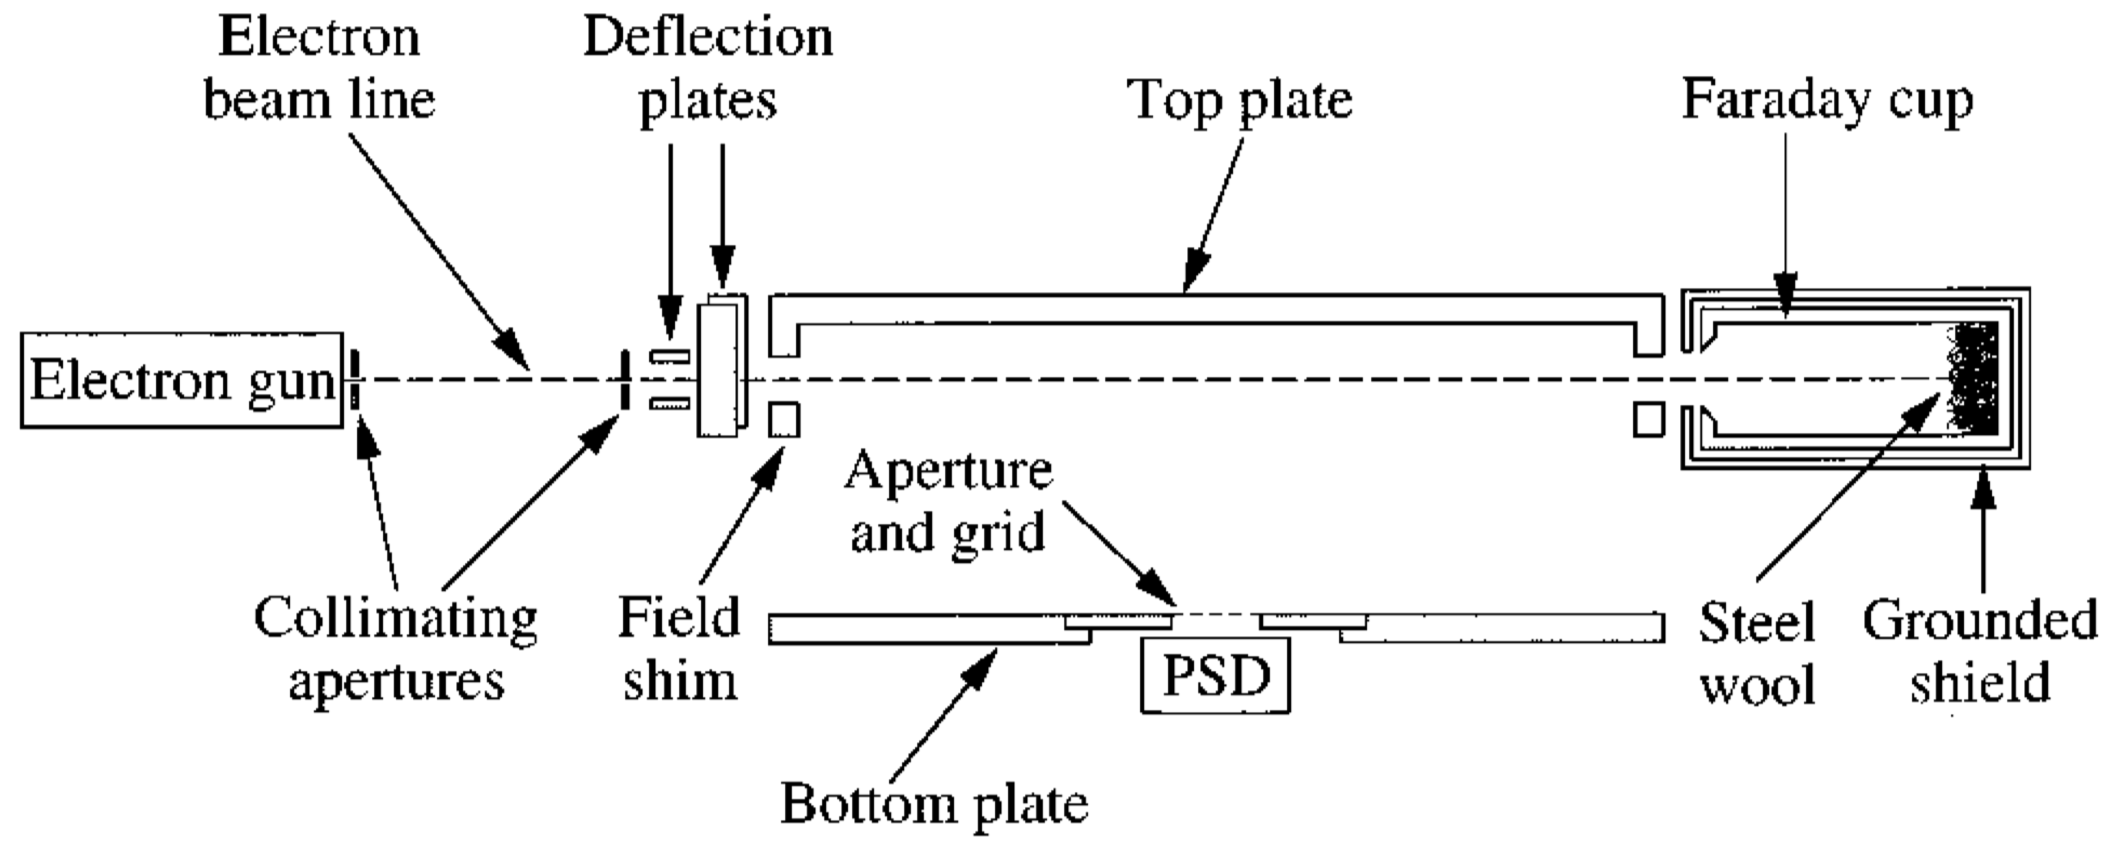
\includegraphics[width=0.85\textwidth]{Straub.png}
    \caption[Anlage zur Messung von Ionisationsquerschnitten von Straub et al.]{Anlage zur Messung von Ionisationsquerschnitten aus \cite{Straub2}. Der Aufbau ähnelt stark dem der in Kapitel \ref{chap:Aufbau} beschriebenen \textsc{Zero-B}-Anlage, mit dem Unterschied, dass die Anlage von Straub et al. eine geringere Flugstrecke zum Detektor hat und auf Linsen verzichtet.}
    \label{fig:Straub}
\end{figure}
Auch die Untersuchung der Elektronenstoßionisation selbst ist seit vielen Jahren ein zentrales Thema in der Atom- und Plasmaphysik. Für die Analyse der in dieser Arbeit gewonnenen Ergebnisse sollen in Kapitel \ref{chap:ion} die physikalischen Grundlagen der Elektronenstoßionisation und die Ansätze für theoretische Beschreibungen der verschiedenen Ionisationsprozesse erläutert werden.